\section{Estados}\label{sec:uc0}


\subsection{Estado del Juego}\label{sec:uc0}

Tenemos que es estado inicial de este diagrama es Juego en ejecución, una vez estamos en este estado tenemos dos opciones, continuar una partida ya existente (partida guardada) o bien, empezar una partida nueva. En ambas situaciones, el proximo estado, es la ejecución de la partida.
  \\
  \\A continuación se pueden dar dos casos, uno de ellos es que se haya acabado el tiempo, y por lo tanto la partida finaliza, posteriormente, se pasa a actualizar el ranking, y se empieza una partida nueva.
  \\
  \\El segundo caso es que sea el jugador quien desee terminar la partida, en esta situación simplemente se sale del juego, y llegamos al estado final.
  \\
  
 \begin{figure*}[ht]
	\centering
	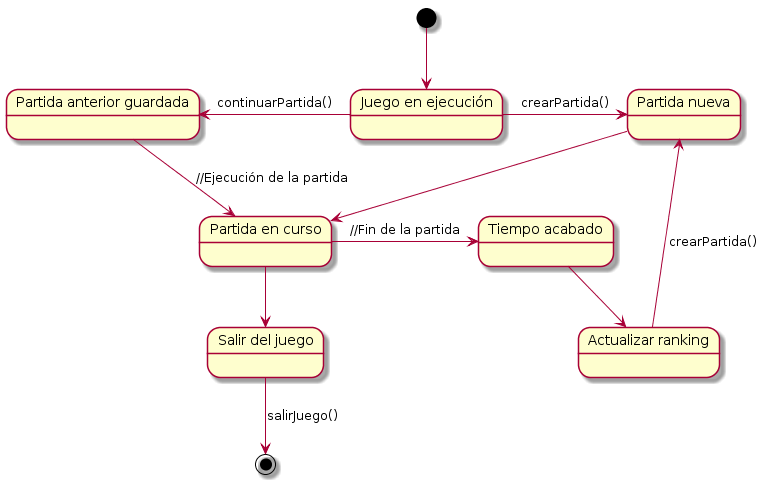
\includegraphics[width=0.9\textwidth]{./imatges/Estados_juego.png}
	\caption{Estado del Juego}
\end{figure*} 


\newpage

\subsection{Partida}\label{sec:uc0}
  Tenemos que es estado inicial de este diagrama es Juego en ejecución, una vez estamos en ejecución solo podemos entrar en una sala. A continuación pueden pasar dos cosas, una es que resolvamos el puzzle y volvemos a entrar en otra sala. Pero también puede pasar que no se consiga resolver el puzzle en el tiempo establecido, y como consecuencia se acaba el juego.
  \\
  \\Una vez acabado el juego, podemos, volver a entrar en una sala (empezar otra partida), o bien, salir del juego, llegando al estado final.
  \\
\begin{figure*}[ht]
	\centering
	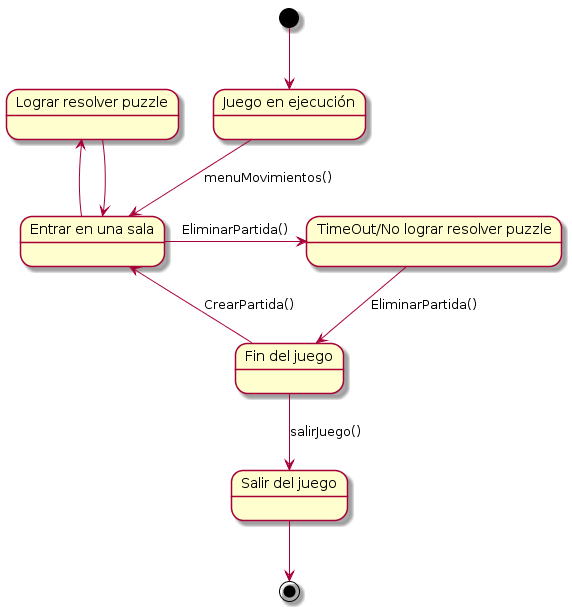
\includegraphics[width=0.8\textwidth]{./imatges/Partida.png}
	\caption{Partida}
\end{figure*}
  
  %\begin{center}
  %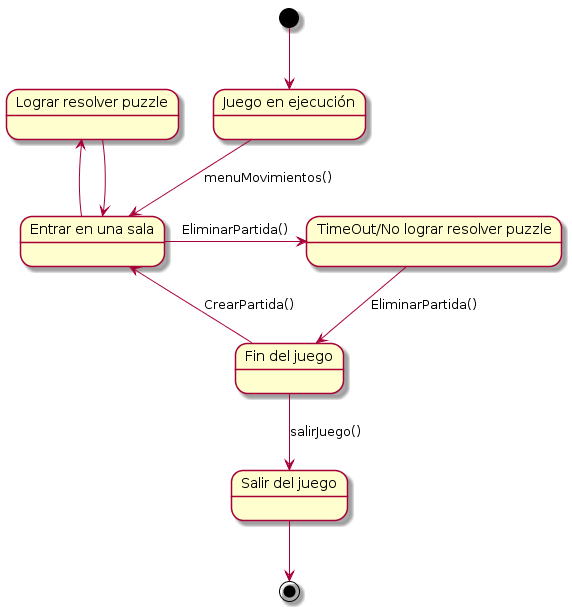
\includegraphics[width=0.9\textwidth]{./imatges/Partida.png}
%\end{center